\section{Příklad 3}
% Jako parametr zadejte skupinu (A-H)
\tretiZadani{H}

%%% Krok 1 - Úprava obvodu
\begin{center}
    \textbf{Krok 1} - Pre jednoduchšie počítanie prevedieme si odpor na vodivosť a napäťové zdroje na prúdové
    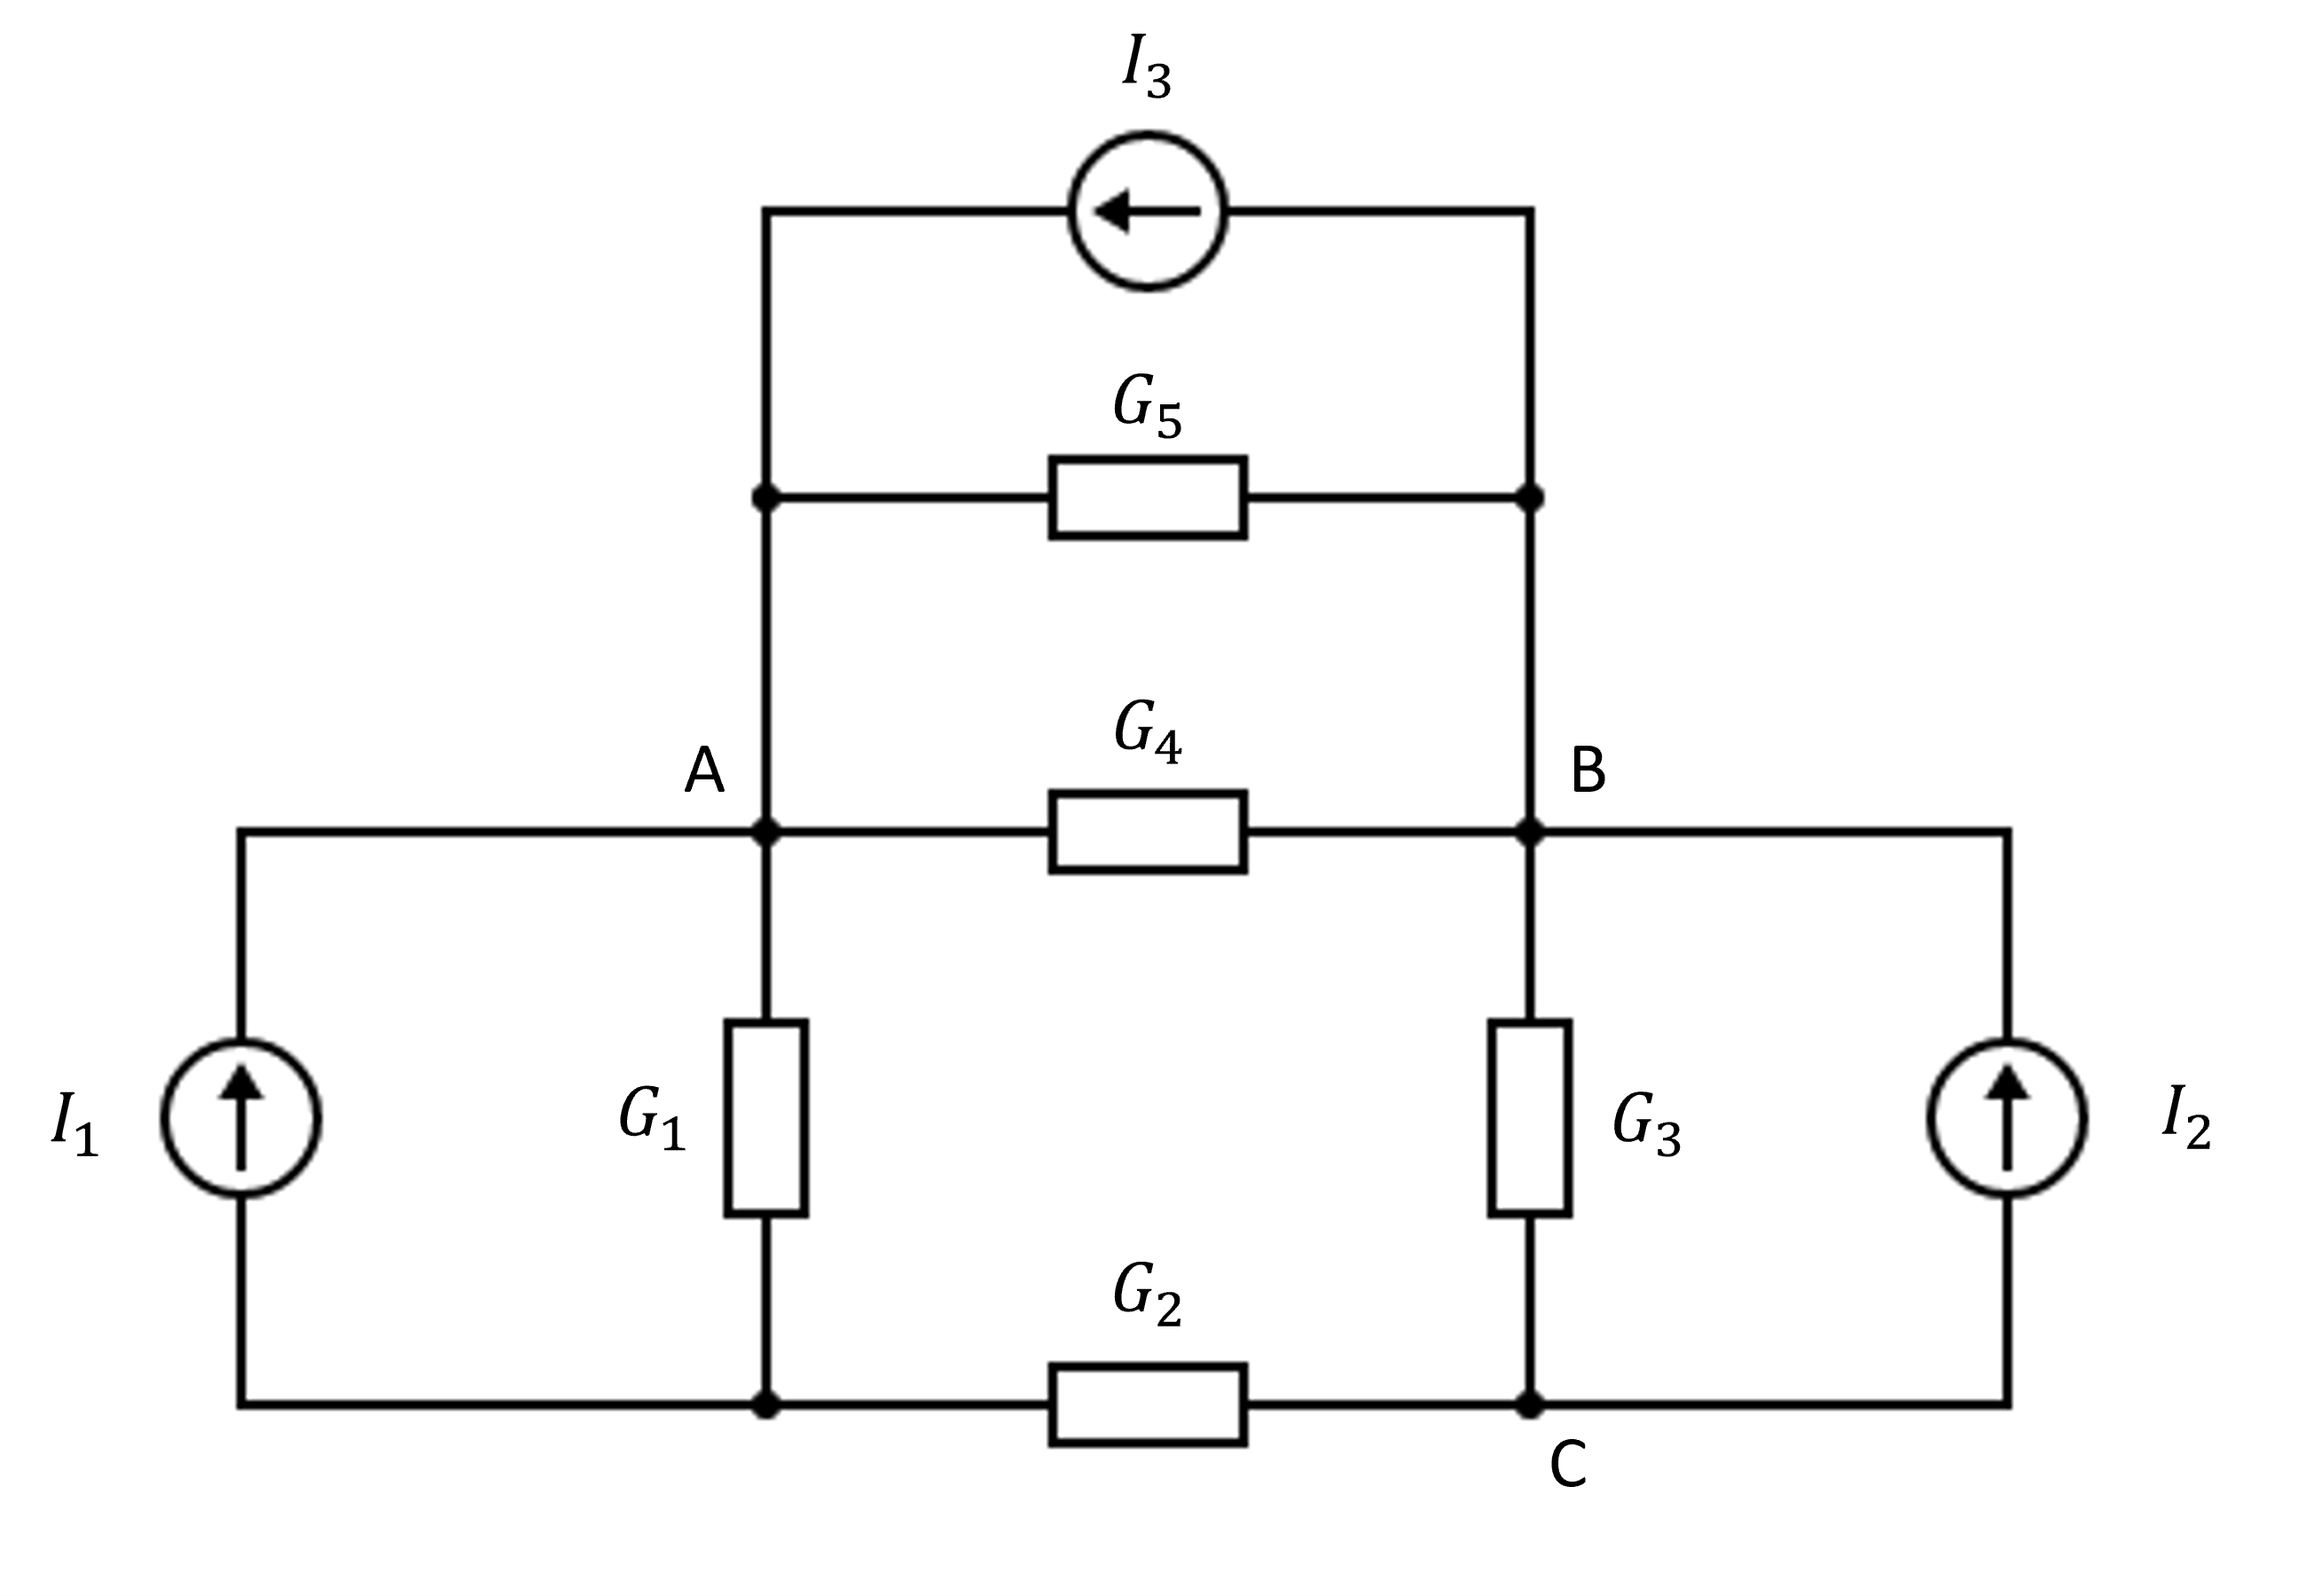
\includegraphics[scale=0.5,keepaspectratio]{fig/pr3_1.png} \\
\end{center}

\begin{gather*}
    G = \frac {1} {R} \\
    I_3 = G_1 \times U = \frac {1} {25} \times 130 = 5,2 A \\
\end{gather*}

\newpage

%%% Krok 2 - Uzlove napatia
\begin{center}
    \textbf{Krok 2} - Pomocou metódy uzlových napätí vypočítame $U_{A}$, $U_{B}$, $U_{C}$ 
\end{center}

\begin{gather*}
   A:  U_A(-G_1 - G_4 - G_5) + U_B(G_4 + G_6) = -I_1 - I_3 \\\\
   B:  U_A(G_4 + G_5) + U_B(-G_4 - G_3 - G_5) + U_C(-G_3) = I_2 + I_3 \\\\
   C:  U_B(G_3) + U_C(G_2 + G_3) = I_2 \\
\end{gather*}

Rovnice prepíšeme do matice: \\

\begin{equation*}
\begin{pmatrix}
-G_1 - G_4 - G_5 & G_4 + G_5 & 0 \\
G_4 + G_5 & -G_4 - G_3 - G_5 & -G_3 \\
0 & G_3 & G_2 + G_3 
\end{pmatrix}
\times
\begin{pmatrix}
U_A \\
U_B \\
U_C 
\end{pmatrix}
=
\begin{pmatrix}
-I_1 - I_3 \\
-I_2 + I_3 \\
I_2
\end{pmatrix}
\end{equation*}
\\

Do matic dosadime hodnoty a neznáme vypočítame pomocou determinantov matic a Cramerového pravidla: \\

\begin{equation*}
\begin{pmatrix}
- \frac {3191} {32900} & \frac {53} {700} & 0 \\\\
 \frac {53} {700} & - \frac {1887} {20300} & - \frac {1}{58} \\\\
0 &\frac {1}{58} & \frac {97} {2262} 
\end{pmatrix}
\times
\begin{pmatrix}
U_A \\\\
U_B \\\\
U_C 
\end{pmatrix}
=
\begin{pmatrix}
-6,15 \\\\
4,7 \\\\
0,5
\end{pmatrix}
\end{equation*}

\begin{gather*}
U_A = 60,504 V \\
 U_B = -3,72 V \\
U_C = 13,15548 V \\
\end{gather*}

\begin{center}
    \textbf{Krok 3} - Pomocou $U_{B}$ a $U_{C}$ vypočítame $U_{R_{3}}$ a $I_{R_{3}}$ 
\end{center}

\begin{gather*}
    U_{R_{3}} = U_C +  U_B = -3,72 + 13,15548 = 9,4355 V \\
    I_{R_{3}} = \frac {U_{R_{3}}} {R_3} = \frac {9,4335} {58} = 0,1627 A
\end{gather*}

